%%%%%%%%%%%%%%%%%%%%%%%%%%%%%%%%%%%%%%%%%%%%%%%%%%%%%%%%%%%%%%%%%%%%%%%%%%%%%%%%
%2345678901234567890123456789012345678901234567890123456789012345678901234567890
%        1         2         3         4         5         6         7         8

%\documentclass[letterpaper, 10 pt, conference]{ieeeconf}  % Comment this line out
% if you need a4paper
%\documentclass[a4paper, 10pt, conference]{ieeeconf}      % Use this line for a4
% paper

\setcounter{topnumber}{6}
\setcounter{bottomnumber}{6}
\setcounter{totalnumber}{10}
\renewcommand{\topfraction}{1}
\renewcommand{\bottomfraction}{1}
\renewcommand{\textfraction}{0}
\renewcommand{\floatpagefraction}{1}

% The following packages can be found on http:\\www.ctan.org
%\usepackage{graphics} % for pdf, bitmapped graphics files
%\usepackage{epsfig} % for postscript graphics files
%%\usepackage{mathptmx} % assumes new font selection scheme installed
%%\usepackage{times} % assumes new font selection scheme installed
%%\usepackage{amsmath} % assumes amsmath package installed
%%\usepackage{amssymb}  % assumes amsmath package installed
%\usepackage{subfigure}
%\usepackage{float}
%
%\restylefloat{figure}

%\title{\LARGE \bf
%	The effect of limb position on myoelectric prosthetic control using linear regression
%}%final name

%\author{ \parbox{3 in}{\centering Huibert Kwakernaak*
%         \thanks{*Use the $\backslash$thanks command to put information here}\\
%         Faculty of Electrical Engineering, Mathematics and Computer Science\\
%         University of Twente\\
%         7500 AE Enschede, The Netherlands\\
%         {\tt\small h.kwakernaak@autsubmit.com}}
%         \hspace*{ 0.5 in}
%         \parbox{3 in}{ \centering Pradeep Misra**
%         \thanks{**The footnote marks may be inserted manually}\\
%        Department of Electrical Engineering \\
%         Wright State University\\
%         Dayton, OH 45435, USA\\
%         {\tt\small pmisra@cs.wright.edu}}
%}

%\author{Simon Bruun, Oliver Thomsen Damsgaard, Martin Alexander Garenfeld, Irene Uriarte}% <-this % stops a space

%\begin{document}
		
%	\maketitle
%	\thispagestyle{empty}
%	\pagestyle{empty}
\begin{center}	
	{\huge\textbf{The effect of limb position on myoelectric prosthetic control using linear regression}}
	
	
	{\large \textbf{Simon Bruun, \textit{Undergrad. Student, AAU}, Oliver Thomsen Damsgaard, \textit{Undergrad. Student, AAU}, Martin Alexander Garenfeld, \textit{Undergrad. Student, AAU}, Irene Uriarte, \textit{Undergrad. Student, AAU}}}
\end{center}
	
	\begin{multicols}{2}

	%%%%%%%%%%%%%%%%%%%%%%%%%%%%%%%%%%%%%%%%%%%%%%%%%%%%%%%%%%%%%%%%%%%%%%%%%%%%%%%%

%		\include{content/aAbstract}
\textbf{\textit{Abstract ---} Electromyography (EMG) is widely used for controlling upper limb prosthetics. However, EMG signals for the same movements change with variations in limb position and this lowers the accuracy in control schemes \cite{Fougner2012}. Most previous studies testing the effect of limb position using classification have found a negative effect in performance. Linear regression is a newer method in control of myoelectric prosthetics, which has proven to yield robust simultaneous and proportional control. A novel approach would be to investigate the limb position effect with regression models. This study investigated the effect of limb position in a linear regression-based control scheme, when using Mean Absolute Value (MAV) and Logarithmic Variance (LogVar) as features. Inertial Measurement Unit (IMU) data was additionally included to improve the performance of the regression models. Twelve able-bodied subjects were recruited for data acquisition, performing four wrist movements in three limb positions. One regression model was build to recognize the different wrist movements under study, taking into account both features. The regressors were tested online in a virtual environment. The results showed that changes in limb position do not affect the control when using a linear regression model. This is opposed to previous studies using classification as control scheme. Inclusion of IMU data shows no significant improvement in performance. Linear regression has the potential to be used in future control schemes for myoelectric prosthetics in daily life tasks.}

\textbf{\textit{Keywords---}surface electromyography, inertial measurement units, simultaneous and proportional myoelectric control, linear regression, lower arm prosthetics.}
	
	%%%%%%%%%%%%%%%%%%%%%%%%%%%%%%%%%%%%%%%%%%%%%%%%%%%%%%%%%%%%%%%%%%%%%%%%%%%%%%%%
	
\section*{INTRODUCTION}%%%%%%%%%%%%%%%%%%%%%%%%%%%%%%%%%%%%%%%%%%%%%%%%%%%%%%%%%%%%%%
		
%		\include{content/bIntroduction}
In recent years the development of EMG controlled upper limb prosthetics has advanced considerably, due to an increased interest in the area along with higher demands for better prosthetics and more precise control \cite{Fougner2012}. In the early years most EMG prosthetics functioned by controlling one degree of freedom (DOF) with on-off control, mainly by linking antagonistic muscles to more than one DOF. This kind of prostheses change between states, due to a switching impulse which cause a state machine to shift its present state. Usually a strong and fast muscle contraction is employed to generate the switching signals. \cite{amsuess2014}
This type of control provided users a way to control more than one DOF, but never simultaneously. The switch-control requires the users to go through the movements of the prosthesis to find the one they wanted to perform. As the switching method was slow and non-intuitive, more complex methods were introduced to the EMG prosthetics scene. Classification methods effectively enabled users to use DOFs more freely because the switching was now replaced by direct recognition of different muscle contractions linked to specific prosthetic movements. However, classification methods proved to be sensitive to real life conditions, e.g. change in limb position, muscle fatigue and sweating \cite{Ison2016}. Introducing regression as a new mapping method in myoelectric prosthetics provided a way to enable both simultaneous and proportional control of multiple DOFs. Regression is able to provide a continuous value for each DOF based on the recorded EMG signal, while a classifier only decides upon a certain class. \cite{hahne2014, jiang2010} \\
This means that classification can only translate a recorded EMG signal to one movement of the prosthetic at a time. It can do so proportionally but the handling still lacks natural control, since movements by able-bodied individuals very rarely only happen in one DOF at a time. Regression methods constantly provide a value, and since several regressors can be used at a time, several values can be used in the recognition of movements. This is what enables regression methods to perform simultaneous and proportional control. 
Applying the regression as a mapping method in proportional and simultaneous control of multiple DOFs has been shown to perform well in recognition of movements and doing so with a low computation time. \cite{hahne2014} A study by Fougner et al. \cite{Fougner2011} has addressed the problem that most studies test their method on only one limb position. This means that the actual performance of regression methods has not yet been properly addressed when recognizing movements, where the arm changes position during daily life tasks. \\
When recording EMG signals it has been shown that some muscles can be activated despite not being directly linked to the performed movement \cite{Fougner2011}. This provides a problem, but can be explained by muscle-synergies \cite{DeRugy2013}. These muscle-synergies are created by the Central Nervous System (CNS) and coordinated into activation of different muscles at varying times. This enables the CNS to control the muscle-synergies instead of controlling each muscle individually to perform movements \cite{jiang2009}. This means that muscles in the lower arm can be activated when muscles in the upper arm are activated, in a level that will be detectable in EMG recordings, and enough to alter recognition of movements, when the arm is active in limb positions other than those tested in a clinical environment. 
In order to overcome the problem of muscles-synergies, Fougner et al. \cite{Fougner2011} has suggested to combine recordings of EMG signals with inertial information to provide limb position data. This could be beneficial in increasing the accuracy of EMG controlled prosthetics for use in daily life tasks. 
Even though the combination of EMG and Inertial Measurement Unit (IMU) data has been proposed as a valid way to improve the performance and accuracy of EMG based prosthetics, it has only been investigated in few studies. \cite{Roy2010, Imtiaz2014, jiang2012} \\
To the authors knowledge the combination of EMG recordings and IMU data has only been done with classification methods. A novel approach to further investigate the usability of combining EMG and IMU is to build a regression based control scheme for myoelectric prosthetics. This would enable both proportional and simultaneous control of several DOFs, where the inclusion of IMU data should provide more information on limb position to counter the effect of limb position.		
	
\section*{METHODS}%%%%%%%%%%%%%%%%%%%%%%%%%%%%%%%%%%%%%%%%%%%%%%%%%%%%%%%%%%%%%%%%%%%
	
%		\include{content/cMethods}
\subsubsection*{Subjects}
For the experiment 12 able-bodied subjects were recruited (10 male, 2 female - 11 right-handed, 1 left-handed. Mean age = 25 $\pm$ 2.05) by contacting fellow undergraduate biomedical engineering students at Aalborg University. All subjects participated in the entire experiment, and were initially informed of the research aim, and instructed about the procedures during the experiment. Entire data sets from three subjects were excluded. The cause for exclusion for these subjects was due to data that did not correspond with the instructed movements. All subjects participated voluntarily, and did not receive any monetary reimbursement. 

To implement online control a number of steps were executed: data acquisition, segmentation, feature extraction and training regression models. The extracted features from the acquired data was used to train the regression models used in online testing.

\subsubsection*{Data acquisition}
EMG signals and inertial information were recorded with the Myo armband from Thalmic Labs - an 8 channel dry electrode armband with 200 Hz EMG sampling rate and 50 Hz IMU sampling rate. The recorded EMG data was filtered using a $2^{nd}$ order Butterworth high-pass filter with a 10 Hz cut-off to remove movement artefacts. Only accelerometer data from the IMU was acquired for data processing. The Myo armband has been suggested as a suitable data acquisition system for pattern classification \cite{Mendez2017}, but not yet for a regression-based control scheme. 
The armband was placed around the thickest part of the dominant forearm, approximately 1/4 of the length of the forearm distal of the elbow. For a close contact between the forearm and armband, clips were used to tighten the fit if necessary. All data acquisition, processing, data analysis and testing was performed in MATLAB (2017b).
In the training data acquisition the subjects were instructed to perform four different wrist movements along 2 DOFs depicted in figure \ref{fig:wristmovement} in three limb positions depicted in figure \ref{fig:limbpositions}. Each movement was performed with four different contraction intensities namely, relaxed, 30\%, 50\% and 80\% of the Maximum Voluntary Contraction (MVC). To ensure that correct fractions of the contraction intensity were recorded, a Graphical User Interface (GUI) was build to provide real-time feedback for the subject. Initially the MVC was recorded and set as reference point for the following trials. \\
The task for the subject was to activate their muscles to track a trapezoidal reference trajectory, where the plateau depicted the desired fraction of the MVC. The level of muscle activation was represented with a cursor, which moved horizontally and continuously with time over 10 s. The vertical position of the cursor was calculated as the mean of the absolute value of the EMG signal across all channels in a 200 ms window, scaled between 0 and 1 according to the MVC. The subject adjusted the height of the cursor by varying the contraction intensity, and was instructed to follow the trapezoidal trajectory as precise as possible. Only the plateau of the trapezoid was used in data processing. The duration of each data acquisition trial was 10 s, where the plateau phase was 3 s. To avoid fatigue the subjects had a 10 s break between trials of different intensities. Between limb position trials subjects were given a 5 min rest. Accelerometer data was additionally recorded in each trial. All trials were performed while standing.
Additional 50\% of MVC EMG data was acquired for each wrist movement in all limb positions to test the accuracy of the regressors on new data. 

\begin{figure}[H]
	\centering
	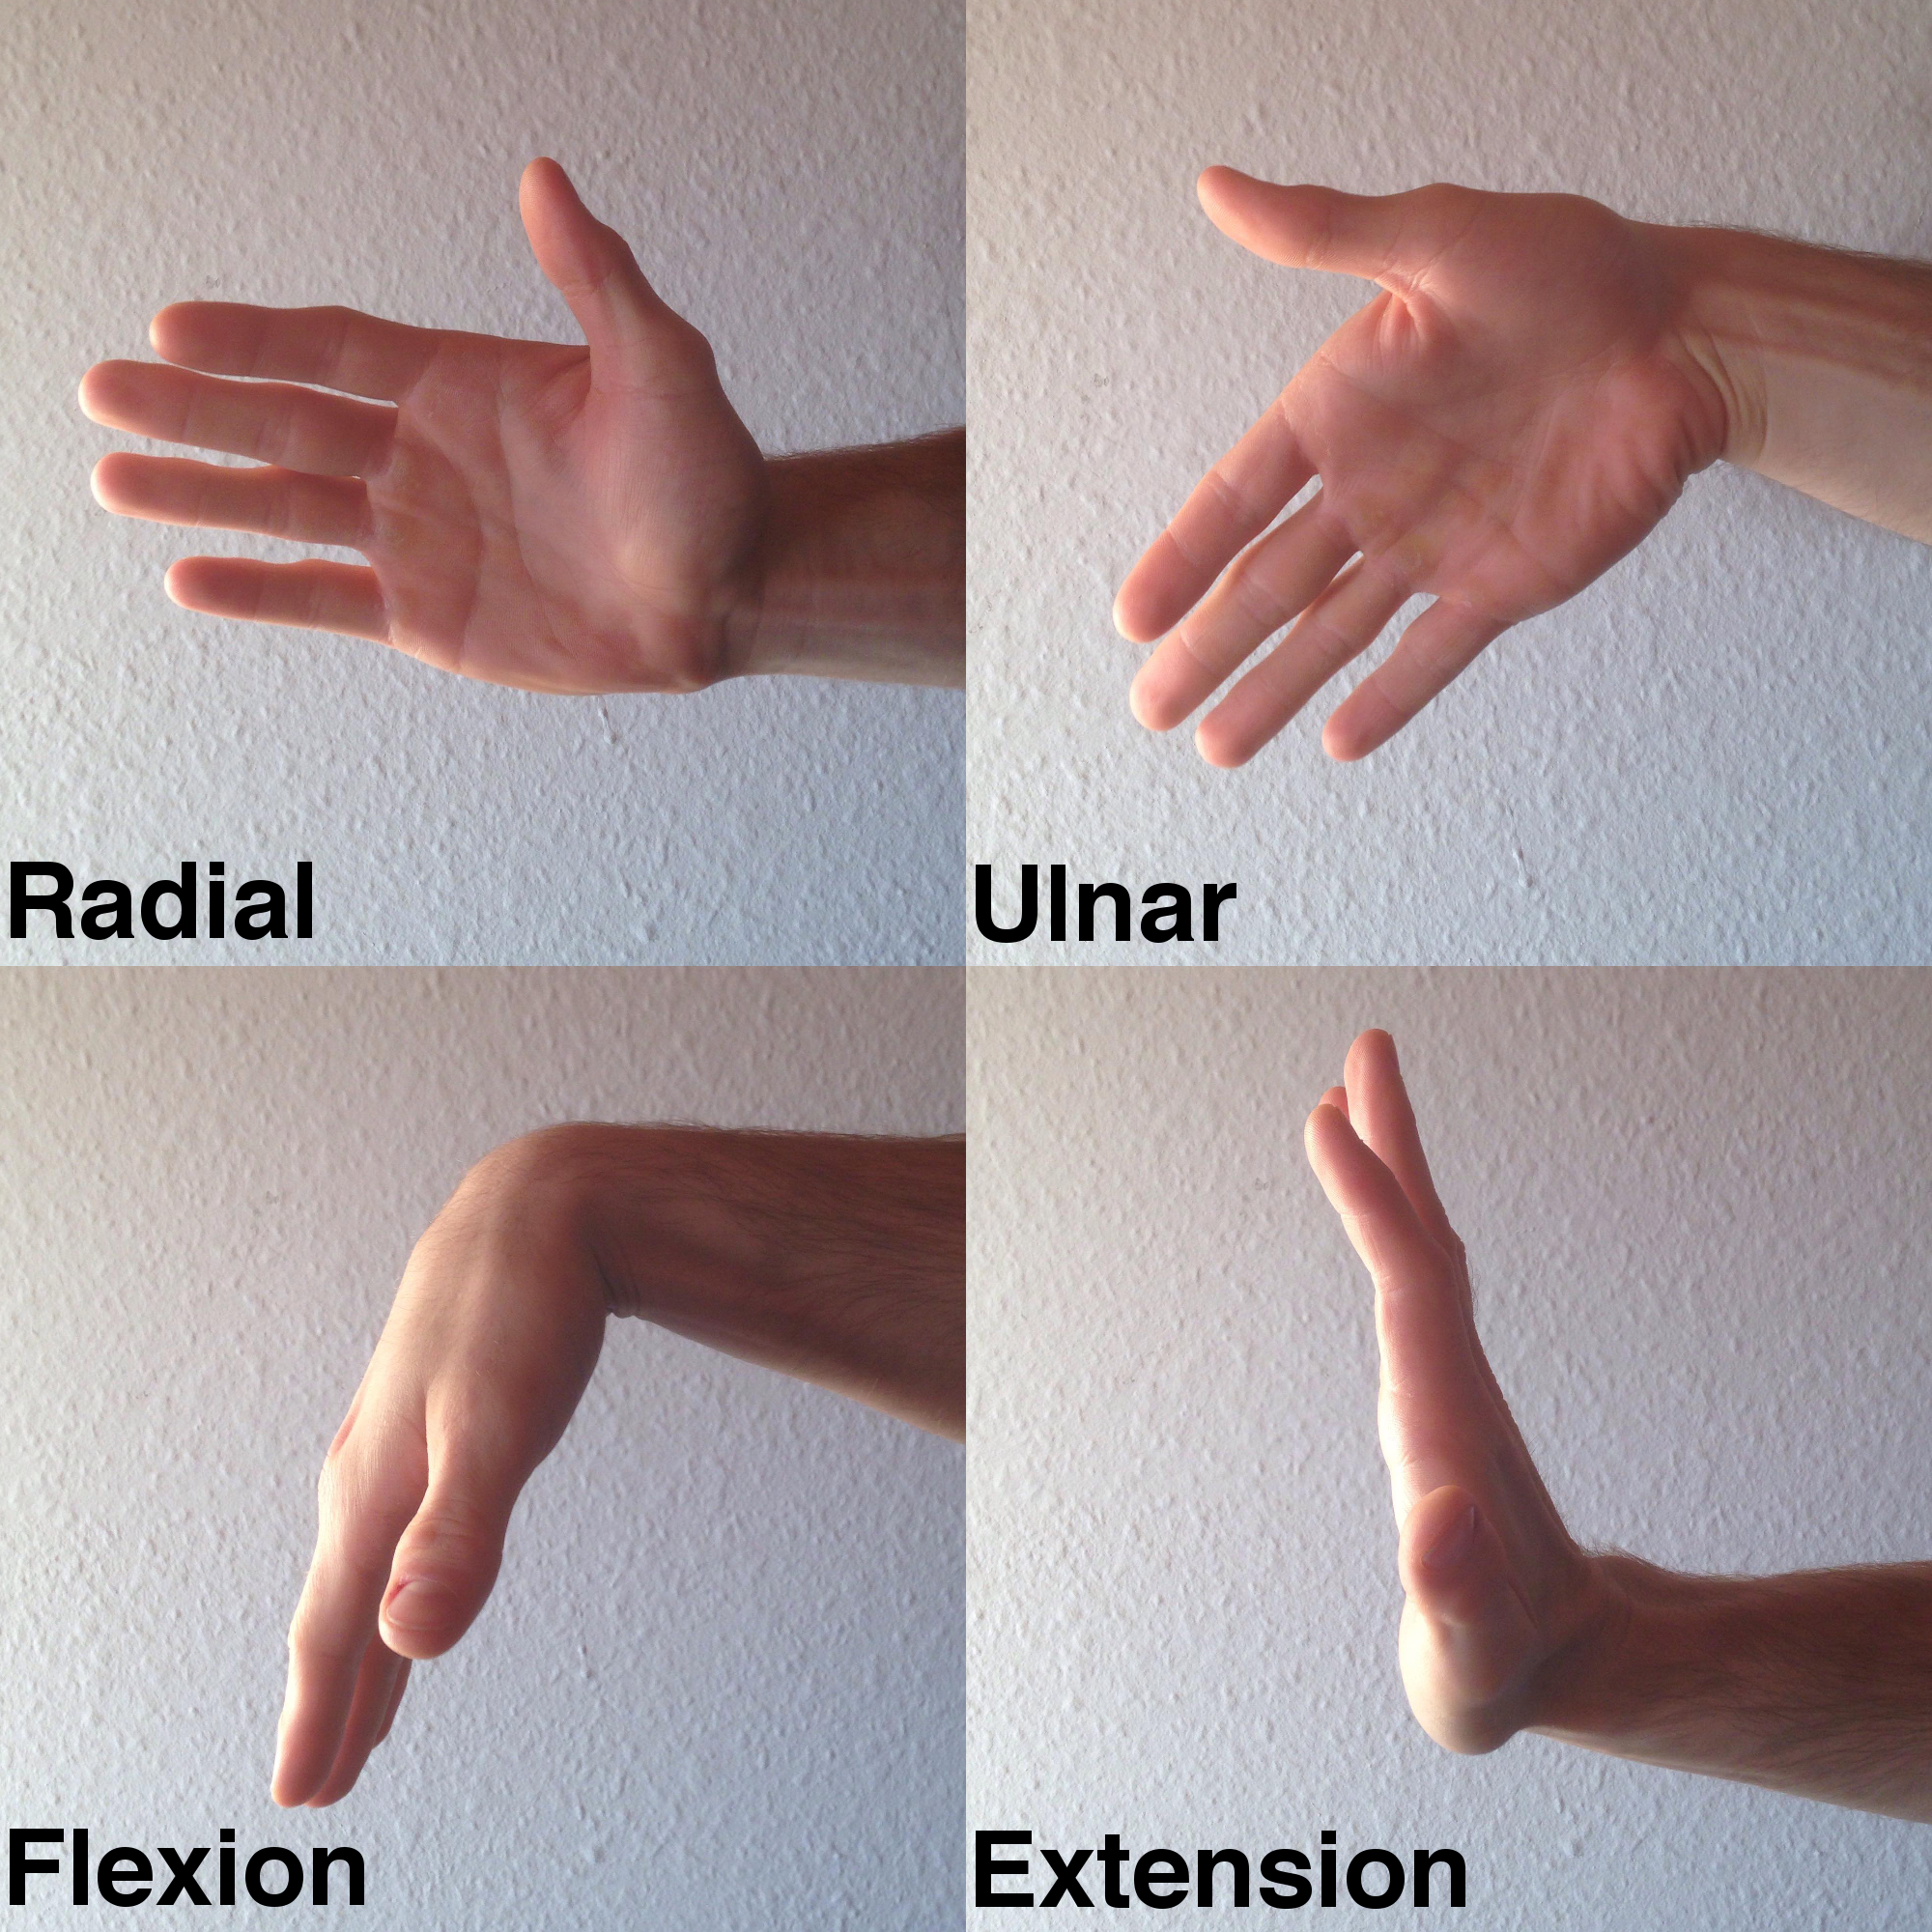
\includegraphics[width=0.4\textwidth]{figures/paperFigures/wristmovement}  %<--but is not needed.
	\caption{Illustration of the two DOFs used in the study.}
	\label{fig:wristmovement}  %<--give the figure a label, so you can reference!
\end{figure}

\begin{figure}[H]
	\centering
	\includegraphics[width=0.45\textwidth]{figures/paperFigures/limb_pos}  %<--but is not needed.
	\caption{Illustration of the limb positions performed. P1: relaxed along the torso, P2: 90\textdegree\  horizontally of the side of torso and P3: 135\textdegree\ vertically in front of the torso.}
	\label{fig:limbpositions}  %<--give the figure a label, so you can reference!
\end{figure}

\subsubsection*{Feature extraction}
The signals were segmented into 200 ms window with a 50\% overlap, which is an acceptable segmentation for preserving information of the signal in static contractions \cite{Farfan2010}.
The commonly used Mean Absolute Value (MAV) feature was additionally extracted, and calculated as given by equation \ref{eq:mav} \cite{Zecca2002}: 

\begin{equation} \label{eq:mav}
MAV = \frac{1}{N}\sum\limits_{i=1}^N|x_i|
\end{equation}
where N is the length of the window, and $x_i$ is the EMG signal of $i^{th}$ sample of the recorded EMG signal.

MAV is directly correlated with change in EMG amplitude. No study has examined whether MAV contains linear properties, but EMG signals has heteroscedastic properties \cite{rasool2012} and the MAV feature might therefore not contain direct linear properties. \\
In a previous study \cite{hahne2014} it was shown that logarithmizing the variance of EMG the feature acquires linear properties, and has yielded robust control of wrist movements in a relaxed limb position when used in linear regression. The Logarithmic Variance (LogVar) was therefore extracted as a feature, and was calculated as given by equation \ref{eq:logvar}:

\begin{equation} \label{eq:logvar}
log(\sigma^2) = log(\frac{\sum\limits_{i=1}^N(x_i - \mu)^2}{N})
\end{equation}
where N expresses the length of the window, $x_i$ is the $i^{th}$ sample of the EMG signal and $\mu$ is the mean.
The extracted EMG features for the individual wrist movements were examined through a Principal Component Analysis, to evaluate, whether the different movements were distinguishable or new training data should be acquired.
The Mean Value (MV) was extracted from the accelerometer data, similarly to a previous study \cite{Krasoulis2015} testing the effect of limb position using classification as control scheme. 

\subsubsection*{Regression model}
As applied in a study by Hwang et al. \cite{Hwang2017} to achieve robust performance across variations in limb positions linear regression was used as control scheme. One regressor was trained for each wrist movement for both features; four regressors trained for each feature, and four for each feature where accelerometer data was included by expanding the dimension of the input matrix. Each regressor was trained based on multivariate linear regression and calculated as given by equation \ref{eq:linearregression}:

\begin{equation} \label{eq:linearregression}
\hat{Y} = \alpha + \beta_1 X_{1} + \beta_2 X_{2} + ... + \beta_i X_{i}
\end{equation}
where $\hat{Y}$ is the control signal value, $X_i$ are the computed features, $\beta_i$ are the regression coefficients in the sampled population, and $\alpha$ is the predicted value of $Y$ at $X_{i} = 0$. For training without inclusion of IMU data $i = 8$ and when including IMU $i = 11$. The control signal was the actual signal the subject generated by tracking the trapezoidal trajectory. The mean of the absolute values of the actual EMG across all channels scaled in relation to the MVC is set as estimator values. The features for all wrist movements in all limb positions were included as predictors in the training of each regressor. However, only the desired wrist movement the regressor was fitted for, was trained with the actual control signal. The remaining predictors were given 0 as control signal. This ensures that the trained regressor will estimate zero when recognising movements other than the one movement it is trained to estimate. This procedure was applied for the regressors to more precisely recognize the performed movement.

\subsubsection*{Offline testing}
The accuracy of the regressors was examined both qualitatively and quantitatively when using both training and test data. A qualitative test was performed by superimposing the estimated signal on the desired signal. The superimposition illustrated whether the right regressor reacted on the performed movement, and how accurate it responded compared to the actual data. For the quantitative analysis the Root Mean Square Error (RMSE) was calculated to compare through statistical analysis, which feature had the lowest error, and whether the regressors were overfitted when tested with new input data. Furthermore, the accuracy of the regressors trained with inclusion of accelerometer data were compared to the regressors trained only using EMG feature data. The RMSE was calculated as given by equation \ref{eq:rmse}:

\begin{equation} \label{eq:rmse}
RMSE = \sqrt{\frac{\sum\limits_{i=1}^N(y_i - \hat{y_i})^2}{N}}
\end{equation}
where N is the length of the window, $y_i$ is the $i^{th}$ variable of the desired signal and $\hat{y_i}$ is the $i^{th}$ estimated signal.

\subsubsection*{Online testing}
To investigate the effect of limb position in the regression control scheme an online virtual environment was developed, depicted in figure \ref{fig:targets}. This approach have also been used on other studies \cite{hahne2014, Hwang2017}.

\begin{figure}[H]
	\centering
	\includegraphics[scale=0.35]{figures/paperFigures/Target}
	\caption{A vector originating from origin depicted vector coordinates calculated from the regressor output, based on the recorded EMG signals. The length of the vector represented the feature intensity, and direction was based on the movement performed.}
	\label{fig:targets}
\end{figure}

In figure \ref{fig:targets} the wrist flexion-extension DOF was mapped to the x-axis, and the radial-ulnar deviation DOF was mapped to y-axis. The vector returned to the target located around origin when no contraction was made. For the subject to reach the targets in the diagonals, a simultaneous movement had to be performed. One target was shown at a time. When a target was reached, the vector had to return to the centred target for a new to appear. This gave the subject the same starting point when reaching each outer target. The procedure was performed until all targets had appeared. If a target was not reached within 30 s, it would disappear, and the vector had to return to the centred target. \\
The time to complete a target-reaching task of sixteen targets was measured. Twelve tests were performed by each subject; one in each limb position for each feature for the regressors trained with and without included accelerometer data. The performance score was calculated as the mean of time per reached target. Time to reach the centred target was not included in the performance score. Performance scores of the online test was compared between the limb positions of the same feature, between all limb positions of the two features and between performance score obtained when using regressors trained with and without inclusion of accelerometer data. The same comparison was additionally applied for the number of targets reached.

\subsubsection*{Statistical analysis}
The statistical analysis was applied for both offline and online results. It was decided, which statistical analysis to apply, through a Kolmogorov-Smirnov test that assesses whether the data populations were normal distributed ($\alpha$ = 0.05). An ANOVA test was applied if the data population belonged to a normal distribution, if not a Friedman's test was applied, which is the non-parametric correspondent to an ANOVA test. 


%\newpage
%\clearpage


\section*{RESULTS}%%%%%%%%%%%%%%%%%%%%%%%%%%%%%%%%%%%%%%%%%%%%%%%%%%%%%%%%%%%%%%%%%%%

The following section contains the offline and online results. The offline results consist of a qualitative and quantitative analysis. The qualitative analysis is based on superimposiion of the estimated signal on the desired signal, while the quantitative analysis is based on the RMSE for different movements for both training and 50\% contraction test data. This comparison is performed to examine the accuracy of the regressors. \\
The online results will focus on the usability of the regressors in the target reaching test, where the results are based on the performance scores and number of targets reached. The performance across limb positions will be compared as well as the performance between the two features. Similar comparison is performed for the regressor with IMU data included. Additionally the usability when including IMU is examined by comparing regressors trained with and without inclusion of IMU data. \\
The Kolmogorov-Smirnov test indicated no dataset to be normal distributed (p < 0.001) in either offline or online data sets. Thus, a Friedman's test was applied for all statistical analysis.

\end{multicols}
\subsubsection*{Offline Results}


\begin{figure}[H]
	\centering
	\subfigure[]{\includegraphics[width=0.90\textwidth]{figures/paperFigures/NewSuperPositionTestDataMAV}}
	\subfigure[]{\includegraphics[width=0.90\textwidth]{figures/paperFigures/NewSuperPositionTestDataLogVar}}
	\caption{Plot of the desired output (red plot) superimposed on the estimate of the regressors trained with the MAV features (a) and LogVar features (b). The plot is divided into four segments, where each segment shows a different movement performed for all limb positions. Each segment has the same sample size and consist of the three contraction intensities.}
	\label{fig:SuperPositionTraining}
\end{figure}

\begin{multicols}{2}
	

A qualitative examination of the superimposition plots in figure \ref{fig:SuperPositionTraining} shows that each regressor reacts on the movement it is fitted for, and remains inactive when another movement is performed. This accounts for both features. However, both regressors has lower accuracy in the high intensities, especially for the regressors trained with LogVar, which outputs similar values for the 80 \% of MVC contractions as the 50 \% of MVC contractions. \\
It is also seen that regressor fitted for the antagonistic movement is more inactive than the other regressors, when the other movement representing that DOF is performed. Furthermore, the regressor output is lower in intensity in all movements above 30\% of the MVC.
	

	\begin{center}
		\scalebox{0.95}{
			\begin{tabular}{l l l}
				\toprule
				\textbf{Feature} & \textbf{Mean error} & \textbf{Std}\\
				\midrule
%				MAV, Extension & 0.1030 & $\pm 0.0210$ \\
%				MAV, Flexion & 0.1102 & $\pm 0.0296$ \\
%				MAV, Radial Dev. & 0.1206 & $\pm 0.0298$ \\
%				MAV, Ulnar Dev. & 0.1143 & $\pm 0.0334$ \\
				MAV training & 0.11 & $\pm 0.03$ \\
				MAV test & 0.17 & $\pm 0.08$ \\
%				LogVar, Extension & 0.1157 & $\pm 0.0469$ \\
%				LogVar, Flexion & 0.1102 & $\pm 0.0241$ \\
%				LogVar, Radial Dev. & 0.1142 & $\pm 0.0256$ \\
%				LogVar, Ulnar Dev. & 0.1312 & $\pm 0.0310$ \\
				LogVar training & 0.12 & $\pm 0.03$ \\
				LogVar test & 0.17 & $\pm 0.06$ \\
				\bottomrule
			\end{tabular}
		}
		\captionof{table}{RMSE for the implemented regression models for both training and test input data.}
		\label{tab:RMSEtrain-test}
	\end{center}
	
	Analysing the RMSE of the regression models' response to the training data, it was found that there was a significant difference (p < 0.01) between MAV and LogVar, where it was shown that LogVar has a higher mean than MAV, as seen in \tabref{tab:RMSEtrain-test}. 
	
	
%	\begin{center}
%		\scalebox{0.85}{
%			\begin{tabular}{l l l}
%				\toprule
%				\textbf{Feature} & \textbf{Mean error} & \textbf{Std}\\
%				\midrule
%%				MAV, Extension & 0.1646 & $\pm 0.0753$ \\
%%				MAV, Flexion & 0.1391 & $\pm 0.0841$ \\
%%				MAV, Radial Dev. & 0.2018 & $\pm 0.0424$ \\
%%				MAV, Ulnar Dev. & 0.1743 & $\pm 0.0905$ \\
%				MAV overall & 0.1700 & $\pm 0.0759$ \\
%%				LogVar, Extension & 0.1552 & $\pm 0.0514$ \\
%%				LogVar, Flexion & 0.1680 & $\pm 0.0508$ \\
%%				LogVar, Radial Dev. & 0.1681 & $\pm 0.0540$ \\
%%				LogVar, Ulnar Dev. & 0.2078 & $\pm 0.0621$ \\
%				LogVar overall & 0.1748 & $\pm 0.0563$ \\
%				\bottomrule
%			\end{tabular}
%		}
%		\captionof{table}{RMSE for test data input for the regression models}
%	\end{center}
	
%	\begin{center}
%		\scalebox{0.85}{
%			\begin{tabular}{l l}
%				\toprule
%				\textbf{Compared features} & \textbf{P-Value}\\
%				\midrule
%				LogVar, MAV & 0.0044 \\
%				LogVar test data, MAV test data & 0.1138 \\
%				LogVar test data, LogVar & 0.0001 \\
%				MAV test data, MAV & 0.000002 \\
%				\bottomrule
%			\end{tabular}
%		}
%		 \label{tab:RMSEp-values}
%		\captionof{table}{P-Values for comparison of the features.}
%	\end{center}
	
	A significant difference was found (p < 0.001) between the RMSE for test data and training data for LogVar. A significant difference (p < 0.001) was also found for the test data and training data for the MAV based regression models, where the test data had the highest RMSE. No significant difference (p = 0.11) was found between MAV and LogVar regression models with test data.
	
\end{multicols}
	
	\subsubsection*{Online Results}
\begin{figure}[H]
	\centering
	\includegraphics[width=1\textwidth]{figures/paperFigures/GotItTimeCol}  %<--but is not needed.
	\caption{Bar chart representing the mean and standard deviation of the performance scores for MAV and LogVar features without (figure A) and with inclusion of IMU data (figure B).}
	\label{fig:GotItTimeCol}
\end{figure}
	
\begin{figure}[H]
	\centering
	\includegraphics[width=1\textwidth]{figures/paperFigures/allRegressorBarzTimeScoreForTargetTestCol}  %<--but is not needed.
	\caption{Figure A shows the bar chart of the overall performance scores for MAV and LogVar features without and with inclusion of IMU data. Figure B shows the overall number of targets reached for MAV and LogVar features without and with inclusion of IMU data.}
	\label{fig:TargetScoresTargetsCol}  %<--give the figure a label, so you can reference!
\end{figure}
	\begin{multicols}{2}
%\newpage

%		\begin{center}
%			\scalebox{0.85}{
%			\begin{tabular}{l l l}
%				\toprule
%				\textbf{Position, feature} & \textbf{PS} & \textbf{Std}\\
%				\midrule
%				Down, MAV & 5.3377 & $\pm 1.5696$ \\
%				Forward, MAV & 8.1791 & $\pm 4.7145$ \\
%				Side, MAV & 6.0490 & $\pm 2.0490$ \\
%				Down, LogVar & 6.5404 & $\pm 2.5315$ \\
%				Forward, LogVar & 7.9123 & $\pm 3.4572$ \\
%				Side, LogVar & 6.9325 & $\pm 2.3036$ \\
%				\bottomrule
%			\end{tabular}
%		}
%			\captionof{table}{Performance score (PS) for the different limb positions for MAV and LogVar regressors.}
%		\end{center}
%
%\begin{center}
%	\scalebox{0.85}{
%		\begin{tabular}{l l}
%			\toprule
%			\textbf{Feature} & \textbf{P-Value}\\
%			\toprule
%			MAV & 0.0319 \\
%			LogVar & 0.4594 \\
%			\toprule
%		\end{tabular}
%	}
%	\captionof{table}{P-Values for comparison of the scores across different limb positions with MAV and LogVar.}
%\end{center}

	
	When comparing the score across limb positions, no significant difference was found for either MAV (p = 0.89) or LogVar (p = 0.24).
	
		\begin{center}
			\scalebox{0.95}{
			\begin{tabular}{l l l}
				\hline
				\textbf{Position, feature} & \textbf{Mean TR} & \textbf{Std}\\
				\hline
				Down, MAV & 15.56 & $\pm 0.73$ \\
				Forward, MAV & 15.11 & $\pm 1.05$ \\
				Side, MAV & 15.22 & $\pm 0.83$ \\
				Down, LogVar & 15.44 & $\pm 0.73$ \\
				Forward, LogVar & 15 & $\pm 1.80$ \\
				Side, LogVar & 15.33 & $\pm 1.12$ \\
				\hline
			\end{tabular}
		}
			\captionof{table}{Targets reached (TR) in the target reaching test with the MAV and LogVar regressors.}
			\label{tab:2}
		\end{center}
	
	
%		\begin{center}
%			\scalebox{0.85}{
%			\begin{tabular}{l l}
%				\toprule
%				\textbf{Feature} & \textbf{P-Value}\\
%				\midrule
%				MAV & 0.2285 \\
%				LogVar & 0.7788 \\
%				\bottomrule
%			\end{tabular}
%		}
%			\captionof{table}{P-Values for comparison of the number of reached targets across different limb positions with MAV and LogVar.}
%		\end{center}
	
	It was shown that there is no significant difference (p = 0.23) between the number of targets reached across limb positions for MAV. No significant difference (p = 0.78) was found between limb positions for LogVar. The mean number of targets reached for both feature regressors across limb positions are written in \tabref{tab:2}.
	
	
	
%		\begin{center}
%			\scalebox{0.85}{
%			\begin{tabular}{l l l}
%				\toprule
%				\textbf{Position,feature} & \textbf{PS} & \textbf{Std}\\
%				\midrule
%				Down, MAV & 4.8661 & $\pm 1.0839$ \\
%				Forward, MAV & 6.1094 & $\pm 3.3852$ \\
%				Side, MAV & 5.5442 & $\pm 3.5847$ \\
%				Down, LogVar & 6.6691 & $\pm 3.0798$ \\
%				Forward, LogVar & 8.7595 & $\pm 4.7969$ \\
%				Side, LogVar & 6.9652 & $\pm 2.9144$ \\
%				\bottomrule
%			\end{tabular}
%		}
%			\captionof{table}{Performance score (PS) for the different limb positions for MAV and LogVar regressors with IMU included.}
%		\end{center}
%	
%		\begin{center}
%			\scalebox{0.85}{
%				\begin{tabular}{l l}
%					\toprule
%					\textbf{Feature} & \textbf{P-Value}\\
%					\midrule
%					MAV & 0.8948 \\
%					LogVar & 0.2359 \\
%					\bottomrule
%				\end{tabular}
%			}
%			\captionof{table}{P-Values for comparison of the performance scores across different limb positions with MAV and LogVar regressors including IMU data.}
%		\end{center}
		
	
	The perforance scores were similar across limb positions for both MAV with IMU included (p = 0.89) and LogVar with IMU included (p = 0.24).
	
	
		\begin{center}
			\scalebox{0.95}{
			\begin{tabular}{l l l}
				\toprule
				\textbf{Position,feature} & \textbf{Mean TR} & \textbf{Std}\\
				\midrule
				Down, MAV & 15.89 & $\pm 0.33$ \\
				Forward, MAV & 15.11 & $\pm 2.32$ \\
				Side, MAV & 15.56 & $\pm 1.33$ \\
				Down, LogVar & 14.78 & $\pm 1.72$ \\
				Forward, LogVar & 13.56 & $\pm 2.19$ \\
				Side, LogVar & 14.11 & $\pm 1.83$ \\
				\bottomrule
			\end{tabular}
		}
			\captionof{table}{Targets reached (TR) in the target reaching test with the MAV and LogVar regressors with inclusion of IMU data.}
			\label{tab:3}
		\end{center}
		
%		\begin{center}
%			\scalebox{0.85}{
%			\begin{tabular}{l l}
%				\toprule
%				\textbf{Compared Features} & \textbf{P-Value}\\
%				\midrule
%				MAV & 0.4966 \\
%				LogVar & 0.0957 \\
%				\bottomrule
%			\end{tabular}
%		}
%			\captionof{table}{P-Values for comparison of the number of targets reached in different limb positions with MAV and LogVar with IMU data included.}
%		\end{center}
	
	No difference were found for number of targets reached for either MAV with IMU included (p = 0.50) or LogVar with IMU data included (p = 0.10), where the mean and std are shown in figure \ref{fig:TargetScoresTargetsCol}. The mean number of targets reached for each limb position with IMU data included is shown in \tabref{tab:3}.

%		\begin{center}
%			\scalebox{0.85}{
%			\begin{tabular}{l l l}
%				\toprule
%				\textbf{Feature} & \textbf{Mean PS} & \textbf{Std}\\
%				\midrule
%				MAV & 6.5219 & $\pm 3.2253$ \\
%				MAV w. IMU & 5.5066 & $\pm 2.8477$ \\
%				LogVar & 7.1284 & $\pm 2.7619$ \\
%				LogVar w. IMU & 7.4646 & $\pm 3.6740$ \\
%				\bottomrule
%			\end{tabular}
%		}
%			\captionof{table}{Average performance score (PS) of the target reaching test for the four regressor designs.}
%		\end{center}
%
%	
%
%		\begin{center}
%			\scalebox{0.85}{
%			\begin{tabular}{l l}
%				\toprule
%				\textbf{Compared features} & \textbf{P-Value}\\
%				\midrule
%				LogVar, MAV & 0.0833 \\
%				LogVar w/ IMU, MAV w/ IMU & 0.5637 \\
%				MAV, MAV w/ IMU & 0.1779 \\
%				LogVar, LogVar w/ IMU & 0.5637 \\
%				\bottomrule
%			\end{tabular}
%		}
%			\captionof{table}{P-Values for comparison of the overall scores of the target reaching tests.}
%		\end{center}

	
	A significant difference could not be proven between the scores of the target reaching test for LogVar with IMU data and MAV with IMU data (p = 0.56), or between the score of LogVar without IMU data and MAV without IMU data (p = 0.08). It was also found that there is no difference between regression models with and without IMU data for both MAV (p = 0.12) and LogVar (p = 0.56). The number of targets reached is illustrated in figure \ref{fig:TargetScoresTargetsCol}.
	
	
		\begin{center}
			\scalebox{0.95}{
			\begin{tabular}{l l l}
				\toprule
				\textbf{Feature} & \textbf{Mean TR} & \textbf{Std}\\
				\midrule
				MAV & 15.30 & $\pm 0.87$ \\
				MAV w/ IMU & 15.52 & $\pm 1.53$ \\
				LogVar & 15.26 & $\pm 1.26$ \\
				LogVar w/ IMU & 14.15 & $\pm 1.92$ \\
				\bottomrule
			\end{tabular}
		}
			\captionof{table}{Average number of targets reached (TR) in the target reaching test for the four regressor designs.}
			\label{tab:averageNoTR}
		\end{center}
	
	
%		\begin{center}
%			\scalebox{0.85}{
%			\begin{tabular}{l l}
%				\toprule
%				\textbf{Compared Features} & \textbf{P-Value}\\
%				\midrule
%				LogVar, MAV & 1 \\
%				LogVar w/ IMU, MAV w/ IMU & 0.0017 \\
%				MAV, MAV w/ IMU & 0.0124 \\
%				LogVar, LogVar w/ IMU & 0.0016 \\
%				\bottomrule
%			\end{tabular}
%		}
%			\captionof{table}{P-Values for comparison of number of targets reached in the target reaching tests.}
%		\end{center}
	
	A significant difference (p < 0.01) was found between targets reached when IMU was included, where LogVar was proven worse than MAV. There was a significant difference (p < 0.01) between LogVar with and without IMU data. The same significant difference (p < 0.05) between MAV with and without IMU data. There was no difference (p = 1) between targets reached with LogVar and MAV when IMU was not included. The mean number of targets reached are written in \tabref{tab:averageNoTR}.
	
\section*{DISCUSSION}%%%%%%%%%%%%%%%%%%%%%%%%%%%%%%%%%%%%%%%%%%%%%%%%%%%%%%%%%%%%%%%%
	
	The aim for this study was to investigate if it is possible to archive proportional and simultaneous control in myoelectric prosthetics across variations in limb positions using linear regression with inclusion of inertial information. This aim will be further discussed in the following section.
	
%		\include{content/eDiscussion}
\textbf{Stability across limb positions.} Without IMU data there was no significant difference between the performance score for either MAV or logVar across limb positions. There was no significant difference between the number of reached targets for MAV or LogVar. This outcome shows that both MAV and LogVar yields stable performance in limb positions in a linear regression-based control scheme. This finding agrees with the recently published study by Hwang et al. \cite{Hwang2017}, who equivalently found stable online performance across limb positions in a linear regression-based control scheme applying RMS as feature.
When including IMU data the MAV based regression model was shown to have no significant difference in scores across limb positions. Same results were yielded for LogVar. There was no significant difference in the amount of targets reached for the MAV trained regressors and the LogVar trained regressors. 

\textbf{Inclusion of IMU data.} The IMU data included in this study was based on a single accelerometer, where it was expected that the Myo armband would give a similar output as long as the subjects were performing both training and testing from the same starting position. Inclusion of the IMU data was shown to yield the same results in the online performance scores, with no significant difference for either MAV or LogVar when comparing regression models trained with and without accelerometer inputs. Inclusion of the IMU data yielded significantly poorer results for the LogVar regression model, while it led to a significant improvement of the MAV regression model when examining the number of reached targets, despite the mean difference being less than one. The inclusion of IMU data could be a subject of further investigation, as the results might be improved by implementing a system capable of measuring the angles of the joints, in order to create a more versatile and usable regression model outside the clinical environment. Including IMU data could additionally be used to select specific regression models, if a system was build with models fitted for each limb position instead of the same regressors for all positions.

\textbf{Comparison of features.} The online results indicated no significant difference between LogVar and MAV in the performance scores both with and without IMU data included. Based on a study \cite{hahne2014} showing LogVar as a feature with linear properties, it would be expected that this feature would perform better in a linear regression model, than a feature which to the authors knowledge has not been proven to be linear. On the contrary it was shown that a significantly higher number of targets was reached with a linear regression models based on the MAV feature with IMU included, compared to the LogVar regression model with IMU included. When IMU data was not included, there was no difference between the number of targets reached in the test.
Further studies within this field should consider examining other features and studying the effect of combining several features in order to further improve performance independent of the limb position.

\textbf{Offline vs. online training.} Offline testing was only done for MAV and LogVar without IMU data included. A significant difference between the two features when testing with training data was archived in the offline test, but no significant difference when using test data. Comparing RMSE of LogVar with training data and RMSE of LogVar with test data there was a significant difference, where RMSE of the test data had the higher mean. Same results were yielded for the MAV trained regressors. The online results yielded robust control across all limb positions, and therefore no apparent correlation between offline and online testing was found. This could be caused by the subjects ability to adjust to a poorer fitted model when given visual feedback while performing the target reaching test. This observation corresponds with findings in another study by Jiang et al. \cite{jiang2010}.

\textbf{Limitations of the study.} This study was based on data from 12 test subjects, where three had to be excluded. One subject was excluded due to misunderstanding the given instructions and thereby creating an unusable set of training and test data. This limited the control of the regression models giving the subject a mean score above 25 s per target reached and average number of reached targets below 10 for all tests.
Two other subjects were excluded as the recorded intensities were not high enough to differ between the baseline and the higher EMG intensity. This caused the regression models to interpret the baseline in the target-reaching test as movements being performed at between 30\% and 70\% of the MVC. 
To improve the validity of the findings more test subjects should be included in future studies within this field. Subjects with transradial amputations should also be taken into consideration if regression based control schemes were to be considered for future use in myoelectric prosthetic devices. 
Using the Myo armband for data acquisition limited the sampling rate to 200 Hz. Only the 0-100 Hz spectrum of the EMG was represented correctly, where frequencies above 100 Hz was affected by aliasing, since an anti-aliasing filter was not implemented. Along with frequency representation limitations, the Myo armband restricted the number and placement of electrodes to eight channels placed at the same distance distal to the elbow joint, where it might be possible to yield better results with a different electrode placement and number of channels. Further studies should implement conventional EMG electrodes and an ADC with a sufficient sample rate, enabling the entire frequency band of EMG signals to be acquired correctly.		
	
\subsection*{CONCLUSION}%%%%%%%%%%%%%%%%%%%%%%%%%%%%%%%%%%%%%%%%%%%%%%%%%%%%%%%%%%%%%%%
	
% 		\include{content/fConclusion}
In conclusion linear regression can be implemented as control scheme in myoelectric prosthetic control to yield performance with no significant difference across variations of limb position. This is opposed to previous studies using classification as control scheme.
 		
	
	%%%%%%%%%%%%%%%%%%%%%%%%%%%%%%%%%%%%%%%%%%%%%%%%%%%%%%%%%%%%%%%%%%%%%%%%%%%%%%%%
	
	
	\subsection*{ACKNOWLEDGMENT}
	
	The authors would like to thank supervisors Strahinja Dosen, Jakob Lund Dideriksen and Lotte N.S. Andreasen Struijk, and the School of Medicine and Health at Aalborg University for providing equipment. Additionally an acknowledgment to the test subjects for participating voluntarily.
	
%			\bibitem{citeKey} author, title, publisher , volume, year
	
%	\begin{thebibliography}{99}				
%		\bibitem{Fougner2012} Fougner, Anders and Stavdahl, Oyvind and Kyberd, Peter J. and Losier, Yves G. and Parker, Philip A., Control of upper limb prostheses: Terminology and proportional myoelectric control a review, IEEE Trans. Neural Syst. Rehabil. Eng., 20, 2012
%		\bibitem{amsuess2014} Amsuess, Sebastian and Goebel, Peter and Graimann, Bernhard and Farina, Dario, Extending mode switching to multiple degrees of freedom in hand prosthesis control is not efficient, 2014
%		\bibitem{Ison2016} Ison, M and Vujaklija, I and Whitsell, B and Farina, D, High-density electromyography and motor skill learning for robust long-term control of a 7-DoF robot arm, IEEE Trans., 24, 2016
%		\bibitem{hahne2014} Hahne, J. M. and Biebmann, F. and Jiang, Ning and Rehbaum, Hubertus and Farina, Dario and Meinecke, F. C. and Muller, K.-R and Parra, L. C., Linear and Nonlinear Regression Techniques for Simultaneous and Proportional Myoelectric Control, IEEE Trans. Neural Syst. Rehabil. Eng., 22, 2014
%		\bibitem{jiang2010} Jiang, Ning and Vujaklija, Ivan and Rehbaum, Hubertus and Graimann, Bernhard and Farina, Dario, Is accurate mapping of EMG signals on kinematics needed for precise online myoelectric control?, IEEE Trans. Neural Syst. Rehabil. Eng., 22, 2014
%		\bibitem{jiang2012} Jiang, Ning and Dosen, Strahinja and Muller, K R and Farina, Dario, Myoelectric Control of Artificial Limbs: Is There a Need to Change Focus?, IEEE Signal Process. Mag., 29, 2012
%		\bibitem{Fougner2011} Fougner, Anders and Scheme, Erik and Chan, Adrian D.C. and Englehart, Kevin and Stavdahl, {\O}yvind, Resolving the limb position effect in myoelectric pattern recognition, IEEE Trans. Neural Syst. Rehabil. Eng., 19, 2011
%		\bibitem{DeRugy2012} de Rugy, A. and Loeb, G. E. and Carroll, T. J., Muscle Coordination Is Habitual Rather than Optimal, J. Neurosci., 32, 2012
%		\bibitem{jiang2009} Jiang, Ning and Englehart, Kevin B. and Parker, Philip A., Extracting simultaneous and proportional neural control information for multiple-dof prostheses from the surface electromyographic signal, IEEE Trans. Biomed. Eng., 56, 2009
%		\bibitem{Roy2010} Roy, Serge H and Cheng, M Samuel, A Combined sEMG and Accelerometer System for Monitoring Functional Activity in Stroke, Vital Heal. Stat. Ser. 20, 17, 2010
%		\bibitem{Imtiaz2014} Imtiaz, U. and Yamamura, K. and Kong, W. and Sessa, S. and Lin, Z. and Bartolomeo, L. and Ishii, H. and Zecca, M. and Yamada, Y. and Takanishi, A., Application of wireless inertial measurement units and EMG sensors for studying deglutition - Preliminary results, Annu. Int. Conf. IEEE Eng. Med. Biol. Soc. IEEE Eng. Med. Biol. Soc., 2014
%		\bibitem{Mendez2017} Mendez, I and Hansen, B W and Grabow, C M and Smedegaard, E J L and Skogberg, N B and Uth, X J and Bruhn, A and Geng, B and Kamavuako, E N, Evaluation of the Myo Armband for the Classification of hand motions, 2017
%		\bibitem{mobarak2014} Mobarak, Michele Pla and Manuel, Juan and Salgado, Guti{\'{e}}rrez, Transient State Analysis of the Multichannel EMG Signal Using Hjorth ' s Parameters for Identification of Hand Movements, Ninth Int. Multi-Conference Comput. Glob. Inf. Technol., 2014
%		\bibitem{Farfan2010} Farf{\'{a}}n, Fernando D and Politti, Julio C and Felice, Carmelo J, Evaluation of EMG processing techniques using Information Theory, Biomed. Eng. Online, 9, 2010
%		\bibitem{Zecca2002} Zecca, M. and Micera, Silvestro and Carrozza, M. C. and Dario, P., Control of Multifunctional Prosthetic Hands by Processing the Electromyographic Signal, Crit. Rev. Biomed. Eng., 30, 2002
%		\bibitem{rasool2012} Rasool, Ghulam and Bouaynaya, Nidhal and Iqbal, Kamran, MUSCLE ACTIVITY DETECTION FROM MYOELECTRIC SIGNALS BASED ON THE AR-GARCH MODEL, 2012
%		\bibitem{Krasoulis2015} Krasoulis, Agamemnon and Vijayakumar, Sethu and Nazarpour, Kianoush, Evaluation of regression methods for the continuous decoding of finger movement from surface EMG and accelerometry, Int. IEEE/EMBS Conf. Neural Eng. NER, 2015
%		\bibitem{Hwang2017} Hwang, Han Jeong and Hahne, Janne Mathias and M{\"{u}}ller, Klaus Robert, Real-time robustness evaluation of regression based myoelectric control against arm position change and donning/doffing, PLoS One, 12, 2017
%	\end{thebibliography}
%	
\end{multicols}
	
	%%%%%%%%%%%%%%%%%%%%%%%%%%%%%%%%%%%%%%%%%%%%%%%%%%%%%%%%%%%%%%%%%%%%%%%%%%%%%%%%
	